\section{Design di dettaglio}

Dopo aver descritto l’architettura del sistema si procede con il design di dettaglio delle sue componenti principali. 
L’approccio progettuale utilizzato combina aspetti Object-oriented, come l’utilizzo dell’interfaccia come astrazione attraverso la quale caratterizzare i componenti, per scatenare comportamenti diversi su entità soggette ad un comune contratto, con elementi di programmazione funzionale pura, quali la tendenza all’impiego di strutture dati immutabili e la riduzione di side effects, favorendo la descrizione lazy della computazione, la separazione fra componente strutturale e comportamentale delle entità ed altri elencati di seguito.


\subsection{Core}
Il motore della simulazione (simulationEngine) consiste in una descrizione monadica delle fasi della simulazione, che prevede l’aggiornamento dei parametri del mondo, il rilevamento e risoluzione delle collisioni fra le entità che lo popolano, la visualizzazione a video del suo stato aggiornato e l’attesa dell’intervallo di tempo prima della successiva iterazione. In questo modo il codice non contiene i side effects invece presenti in un’equivalente versione procedurale, e la parte non funzionalmente pura, ovvero quella non che rispetta le proprietà di trasparenza referenziale) è situata all’avvio della simulazione. 
Questo andamento sequenziale e periodico è stato modellato attraverso una composizione di State monad  (State[World, A]) (per quanto riguarda l’aggiornamento della struttura del mondo) e di IO monad (per le operazioni di I/O come il display a video delle entità e delle statistiche storiche alla chiusura dell’applicazione). Per tale motivo (e a fini di leggibilità sono stati definiti i seguenti type alias):


\subsection{Model}


\begin{figure}[h!]
\centering
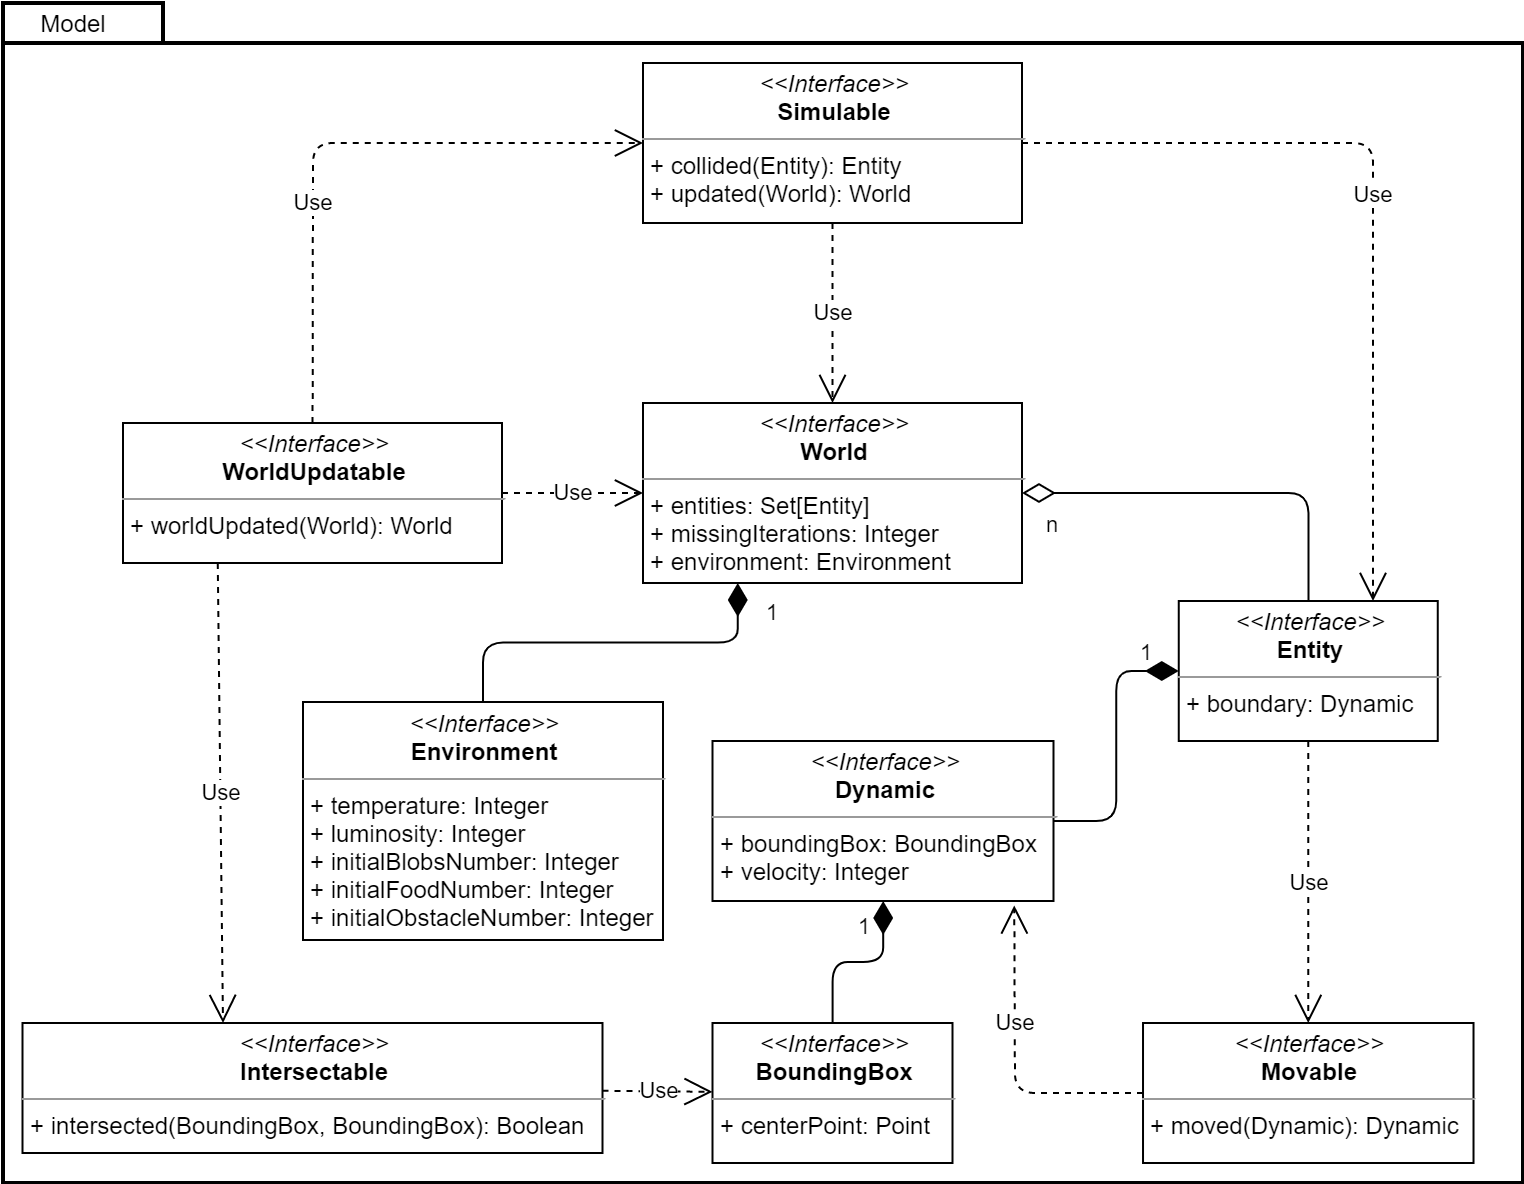
\includegraphics[width=\textwidth, scale=0.44]{img/Model.png}
\caption{Design Model}
\label{fig:model}
\end{figure}

\begin{figure}[h!]
\centering
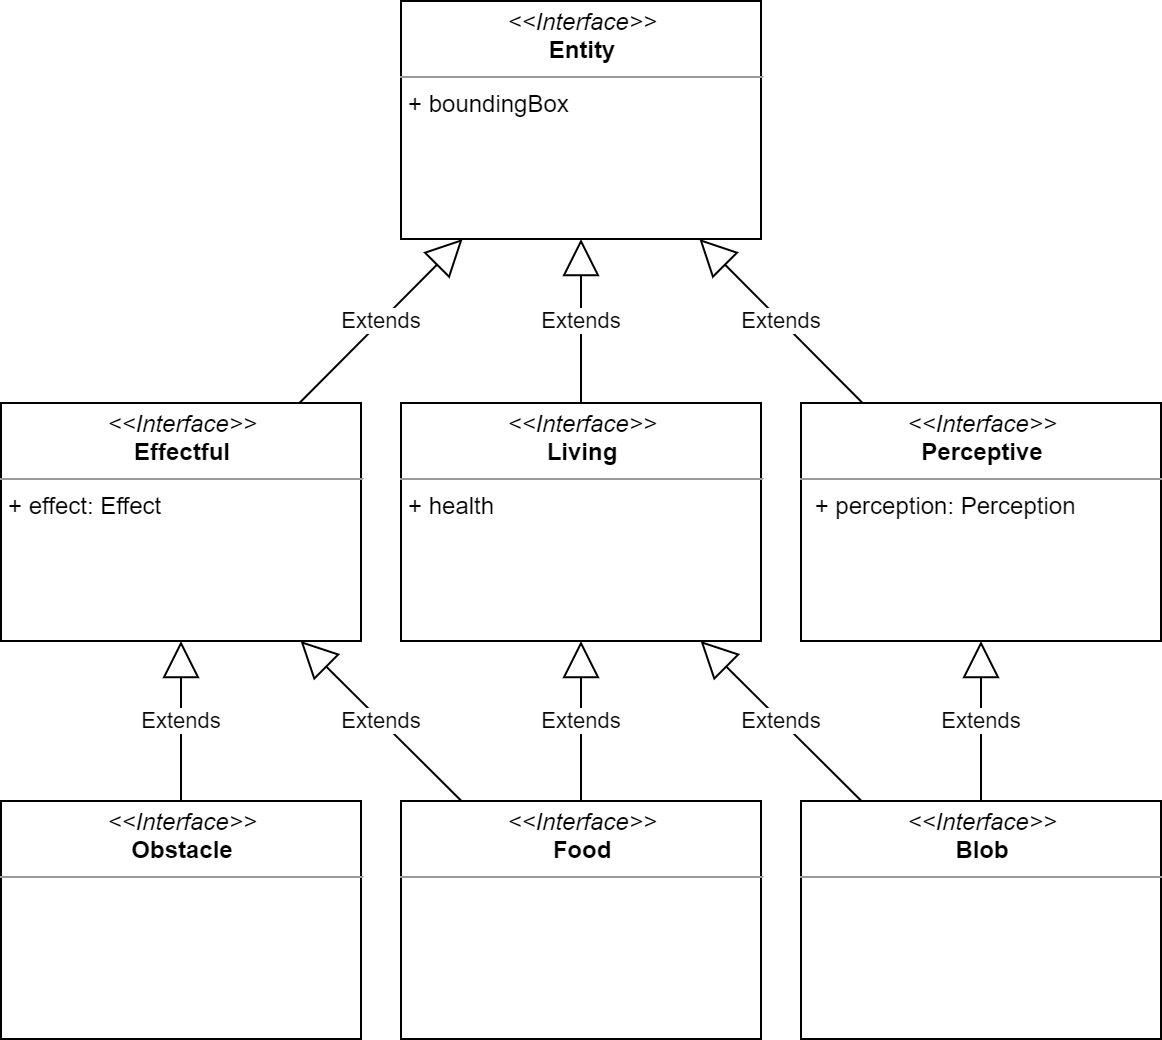
\includegraphics[width=\textwidth, scale=0.44]{img/ModelHierarchy.png}
\caption{Gerarchia Model}
\label{fig:modelhierarchy}
\end{figure}